%%%%%%%%%%%%%%%%%%%%%%%%%%%%%%%%%%%%%%%%%
% University/School Laboratory Report
% LaTeX Template
% Version 3.1 (25/3/14)
%
% This template has been downloaded from:
% http://www.LaTeXTemplates.com
%
% Original author:
% Linux and Unix Users Group at Virginia Tech Wiki 
% (https://vtluug.org/wiki/Example_LaTeX_chem_lab_report)
%
% License:
% CC BY-NC-SA 3.0 (http://creativecommons.org/licenses/by-nc-sa/3.0/)
%
%%%%%%%%%%%%%%%%%%%%%%%%%%%%%%%%%%%%%%%%%

%----------------------------------------------------------------------------------------
%	PACKAGES AND DOCUMENT CONFIGURATIONS
%----------------------------------------------------------------------------------------

\documentclass{article}

\usepackage{siunitx} % Provides the \SI{}{} and \si{} command for typesetting SI units
\usepackage{graphicx} % Required for the inclusion of images
%\usepackage{natbib} % Required to change bibliography style to APA
\usepackage{amsmath} % Required for some math elements 
\usepackage[margin=1.5in]{geometry}


\setlength\parindent{0pt} % Removes all indentation from paragraphs

\renewcommand{\labelenumi}{\alph{enumi}.} % Make numbering in the enumerate environment by letter rather than number (e.g. section 6)

%ustawienie jezyka polskiego
\usepackage{polski}
\usepackage[utf8]{inputenc}
\usepackage[T1]{fontenc}
\usepackage{multirow}
\usepackage{rotating}
\usepackage{float}
\usepackage[table]{xcolor}
\usepackage{enumerate}
\usepackage{subcaption}


\graphicspath{ {images/} }


%----------------------------------------------------------------------------------------
%	DOCUMENT INFORMATION
%----------------------------------------------------------------------------------------

\title{Projekt z rozproszonych i obiektowych systemów baz danych\\
	\vspace{5mm}
	\textbf{Projekt aplikacji wykorzystującej repliki MongoDB}
	}

\author{\\
	\\\textbf{Autorzy:}
	\\Maciej Kiedrowski, nr indeksu: 200105
	\\Joanna Piątek, nr indeksu: 199966
	\\\\
	\\
	\\\textbf{Grupa:} Poniedziałek 16:10}
\date{\textbf{Data oddania:} 23.01.2017}

%%\newcommand{\myparagraph}[1]{\paragraph{#1}\mbox{}\\}
%%\date{\today} % Date for the report

\begin{document}

\maketitle % Insert the title, author and date

\begin{center}
\begin{tabular}{l r}
\\\\\\
\textbf{Prowadzący zajęcia:} & Dr inż. Robert Wójcik, W4/K-9 \\
\\\textbf{Ocena pracy:} &  %
\end{tabular}
\end{center}
 
\newpage
\tableofcontents 	%spis tresci
\newpage
\listoffigures
\newpage

%-----------------------------------------------------------
\section{Wstęp}
Niniejszy projekt realizowany w ramach kursu "Rozproszone i obiektowe systemy baz danych" ma na celu zaprojektowanie oraz imlementację rozproszonej aplikacji, odpornej na awarię baz danych, pozwalającącej zarządzać stanem magazynowym oraz sprzedażą w sieci restauracji.

\subsection{Cele projektu}
Celem projektu jest stworzenie systemu pozwalającego zarządzać siecią restauracji. System pozwala na utworzenie nowej restauracji w bazie, utworzenie menu wspólnego dla całej sieci, zarządzania stanem magazynowym poszczególnych restauracji, sprzedaż prodóktów wpływający na stan magazynowy. Dane o wszystkich restauracjach przechowywane są we wspólnej, centralnej bazie danych - wymaga ona maksymalnej dostępności oraz ochrony danych przed ich utratą. \\
Dostęp do systemu możliwy jest poprzez dowolną przeglądarkę internetową - użytkownik za pomocą interfejsu webowego posiada możliwość wykonywania operacji na bazie danych za pośrednictwem aplikacji serwerowej.
strukturaSystemu

\begin{figure}[H]
	\centering
	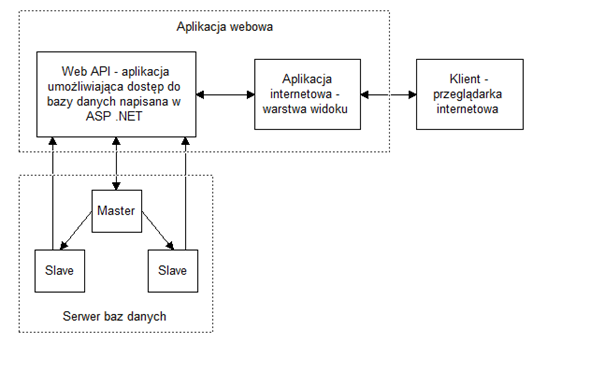
\includegraphics[width=\textwidth]{strukturaSystemu}
	\caption{Struktura systemu i schemat komunikacji}
\end{figure}


\subsection{Założenia projektowe}
Jako silnik bazy danych wybrany został system MongoDB ze względu na skalowalność, wydajność oraz architekturę zaprojektowaną z myślą o łatwej replikacji. Utworzone zostały trzy serwery bazy danych tworzące zestaw replik MongoDB. Webowa aplikacja kliencka został wykonana w oparciu o platformę ASP .NET MVC. 


\newpage
\section{Replikacja}
Proces replikacji polega na synchronizacji danych pomiędzy serwerami. Pozwala osiągnąć następujące korzyści:
\begin{itemize}
	\item Bezpieczeństwo danych poprzez renundancję
	\item Wysoką dostępność
	\item Skalowanie wydajności
\end{itemize}

\subsection{Replikacja w MongoDB}
Replikacja wbudowana w platformę \textit{MongoDB} opiera się na \textit{replica set} - zestawie replik.

\subsubsection{Zestaw replik}
\begin{description}
\item[Zestaw replik]
 grupa procesów \textit{mongod} utrzymujących ten sam zestaw danych. Zestaw replik w ramach MongoDb skłąda się z węzłów zawierającyh dane oraz ewentualnego węzłą wspomagającego arbitraż.
\end{description}

\begin{figure}[H]
	\centering
	\begin{subfigure}{.5\textwidth}
		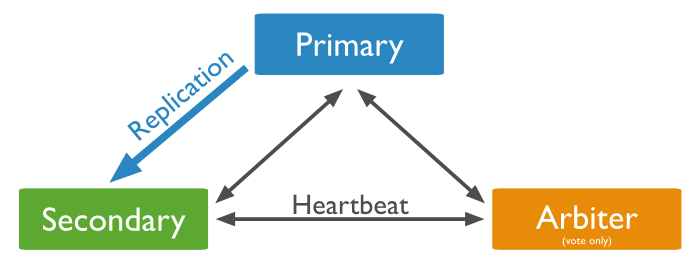
\includegraphics[scale=0.5]{arbiter}
		\label{fig:sub2}
	\end{subfigure}
	\caption{Zestaw replik}
	\label{fig:test}
\end{figure}

W każdym zestawie replik jeden z węzłów pełni rolę \textit{Primary}. Węzeł ten jest jedynym, który akceptuje operacje zapisu, jest również domyślnym węzłem dla wszystkich operacji odczytu z zestawu replik. Pozostałe węzły wchodzące w skład zestawu, a niebędące węzłem arbitrażowym działają w trybie \textit{Secondary}. Minimalna ilość węzłów zapewniająca poprawną pracę zestawu to 3, ilośc węzłów powinna być nieparzysta.

\begin{figure}[H]
	\centering
	\begin{subfigure}{.5\textwidth}
		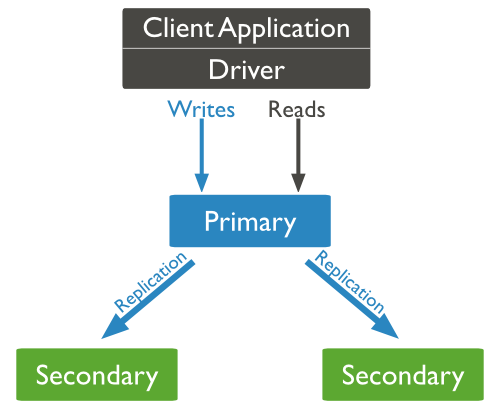
\includegraphics[scale=0.5]{replica-set-read-write-operations-primary}
		\label{fig:sub2}
	\end{subfigure}
	\caption{Shemat działania zestawu replik}
	\label{fig:test}
\end{figure}


\subsubsection{Replikacja} 
Replikacja w \textit{MongoDB} jest replikacją asynchroniczą. Węzły \textit{Secondary} replikują dziennik operacji (\textit{oplog}) węzła \textit{Primary} i wykonują operacja w nim zawarte na przechowywanym zbiorze danych.

\subsubsection{Wysoka dostępność}
Zestawe replik gwarantuje wysoką dostępność danych. W przypadku awarii węzła, w szczególności węzła \textit{Primary} uruchamiany jest proces \textit{failover}. Ma on na celu zapewnienie płynności dostępu do danych. Pozostałe dziłające węzły w ramach repliki przeprowadzają głosowanie nad wyborem nowego \textit{Primary}, po zakończeniu głosowania zestaw odzyskuje pełną sprawność. Proces \textit{failover} trwa przeważnei poniżej minuty, z czego 10-30 sekund to wykrycie awarii węzła \textit{Primary}, następne 10-30 sekund proces głosowania. \\
W trakcie głosowania zestaw pracuje w trybie \textit{read-only} - żaden z węzłów nie posiada statusu \textit{Primary} a zatem wszystie żądania zapisu do bazy są odrzucane. \\

\begin{figure}[H]
	\centering
	\begin{subfigure}{.5\textwidth}
		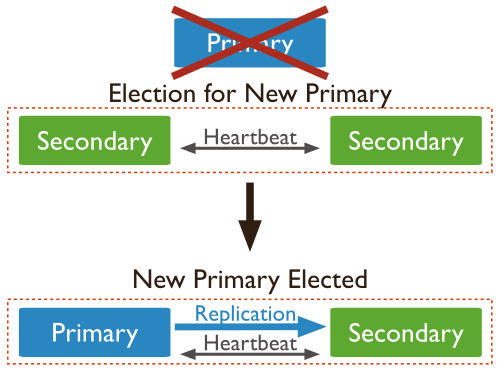
\includegraphics[scale=0.5]{replica-set-trigger-election}
		\label{fig:sub2}
	\end{subfigure}
	\caption{Wysoka dostępność z wykorzystaniem procesu \textit{failover}}
	\label{fig:test}
\end{figure}

Warunkiem koniecznym do istnienia węzła \textit{Primary} w zestawie, jest dostępność ponad 50\% węzłów. Oznacza to, że dla zestawu składającego się z 3 instancji, jest on w pełni funkcjonalny przy awarii 1 węzła, natomiast zestaw skłądający się z 5 węzłów pozwala na awarię 2 węzłów. \\
W przypadku dostępnośći mniejszej liczby węzłów w zestawie, wszystkie pozostałe przechodzą w tryb \textit{Secondary} - zestaw działa w trybie \textit{read-only}. Mechanizm ten służy zabezpieczeniu danych przed brakiem lub niewystarczającą replikacją w systemie.

\subsubsection{Dostępność}
Poprawne działanie węzłów monitorowane jest za pomocą \textit{Heartbeats}. Instancje co 2 sekundy wzajemnie informują się o poprawnym działaniu, brak informacji przez 10 sekund traktowany jest jako awaria węzłą.

\begin{figure}[H]
	\centering
	\begin{subfigure}{.5\textwidth}
		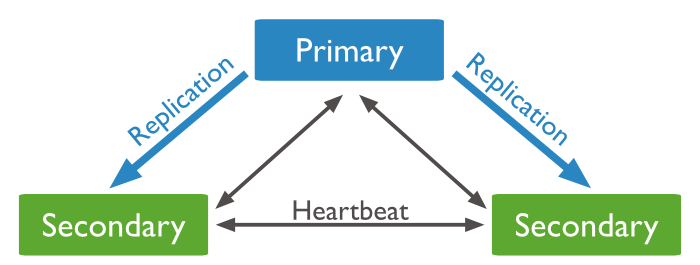
\includegraphics[scale=0.5]{heartbeats}
		\label{fig:sub2}
	\end{subfigure}
	\caption{Monitorowanie działania węzłów}
	\label{fig:test}
\end{figure}

\newpage
\section{Analiza wymagań}

\subsection{Model konceptualny}

\begin{figure}[H]
	\centering
	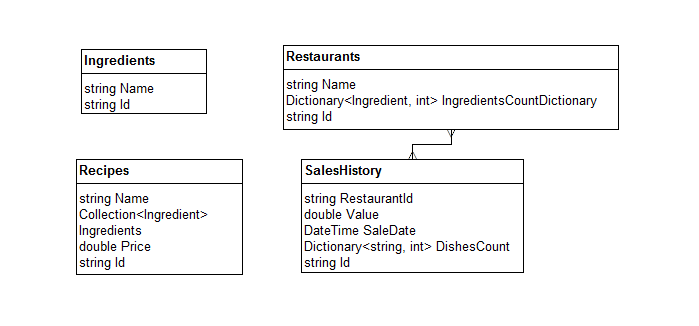
\includegraphics[width=\textwidth]{modelKonc}
	\caption{Model konceptualny bazy danych}
	\label{rys:modelKonc}
\end{figure}


\subsection{Model fizyczny}

\begin{figure}[H]
	\centering
	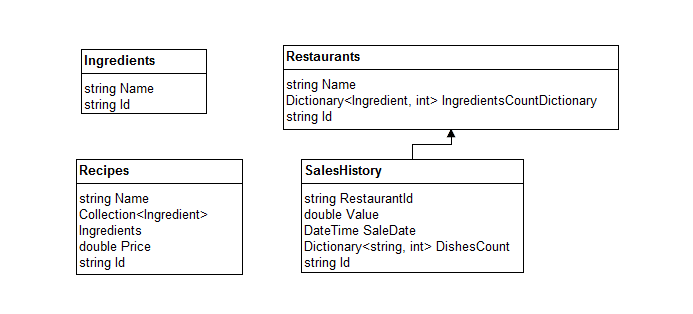
\includegraphics[width=\textwidth]{modelFiz}
	\caption{Model konceptualny bazy danych}
	\label{rys:modelFiz}
\end{figure}
\newpage
\section{Implementacja bazy danych w środowisku MongoDB}
Celem implementacji było stworzenie zestawu replik skłądającego się z 3 procesów \textit{mongod} działających na niezależnych instancjach. 

\subsection{Infrastruktura}
\subsubsection{Instancje}
Baza danych oparta została o chmurę \textit{Azure} w modelu IaaS - \textit{infrastruktura jako usługa}.\\
Utworzone zostały 3 maszyny wirtualne z wykorzystanim obrazów dostarczanych przez \textit{Bitnami}. Systemem operacyjnym działającym na maszynach wirtualnych jest Ubuntu 14.04, natomiast wersja MongoDB to 3.2.9. \\

\subsubsection{Sieć wewnętrzna}
Maszyny wirtualne zostały połączone przez prywatną sieć wirtualną, zilustrowaną poniżej. 

\begin{figure}[H]
	\centering
	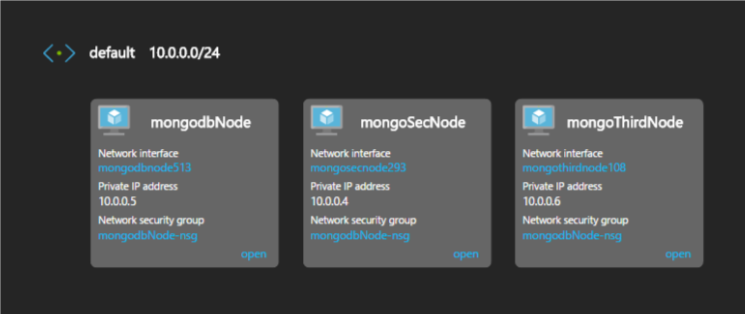
\includegraphics[scale=0.5]{privateNetwork}
	\caption{Sieć wirtualna}
	\label{fig:test}
\end{figure}

\subsubsection{Sieć publiczna}
Aby umożliwić połączenie z zestawem replik od dowolnego klienta, bez wymogu jego wdrożenia w chmurze \textit{Azure}, każdej z instancji maszyn wirtualnych został przydzielony publiczny adres IP, oraz nazwa DNS umożliwiająca dostęp do maszyn.

\subsection{Konfiguracja MongoDB}
Korzystając z \textit{mongo shell} utworzony został zestaw replik oraz jego konfiguracja. 

\begin{figure}[H]
	\centering
	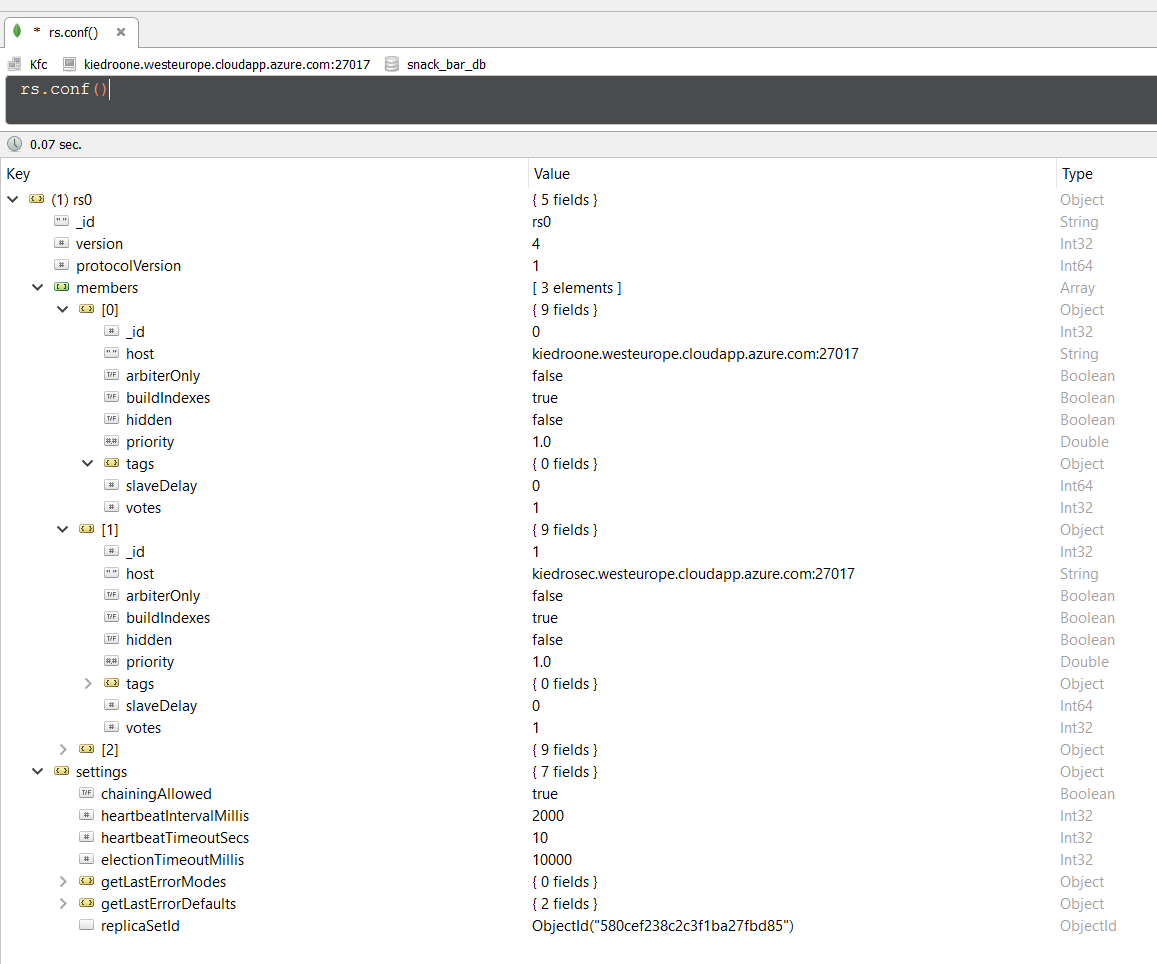
\includegraphics[width=\textwidth]{rsConfig}
	\caption{Konfiguracja zestawu replik}
\end{figure}

Korzystając z pliku konfiguracyjnego uaktywiono prosty interfejs REST, pozwalający na łatwą diagnozę zestawu replik.

\begin{figure}[H]
	\centering
	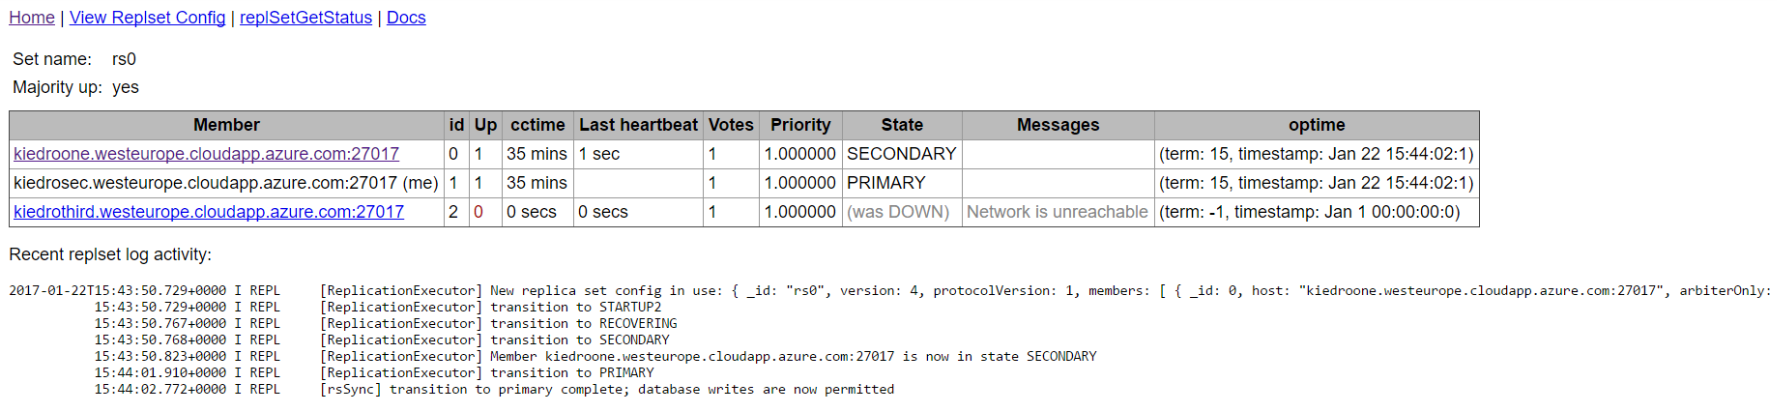
\includegraphics[width=\textwidth]{rest_interface}
	\caption{Interfejs REST}
\end{figure}

\subsection{Schemat bazy danych}
MongoDB należy do baz NoSQL typu dokumentowego, jedną z cech charaktrystycznych baz tego typu jest brak ustalonego schamatu bazy danych. Kolekcje tworzone dynamicznie w trakcie działania aplikacji pozwalają na przechowywanie dowolnych danych - jedynym warunkiem jest możliwość ich serializacji w formacie JSON. \\
Ta cecha baz NoSQL upraszcza wstępną konfigurację bazy danych.

\subsection{Weryfikacja}
Do weryfikacji poprawnego działania bazy danych - możliwości połączenia ze wszystkimi węzłami, odczytu, zapisu, działania mechanizmu replikacji posłużyło narzędzie \textit{Robomongo} w wersji 0.9.

\begin{figure}[H]
	\centering
	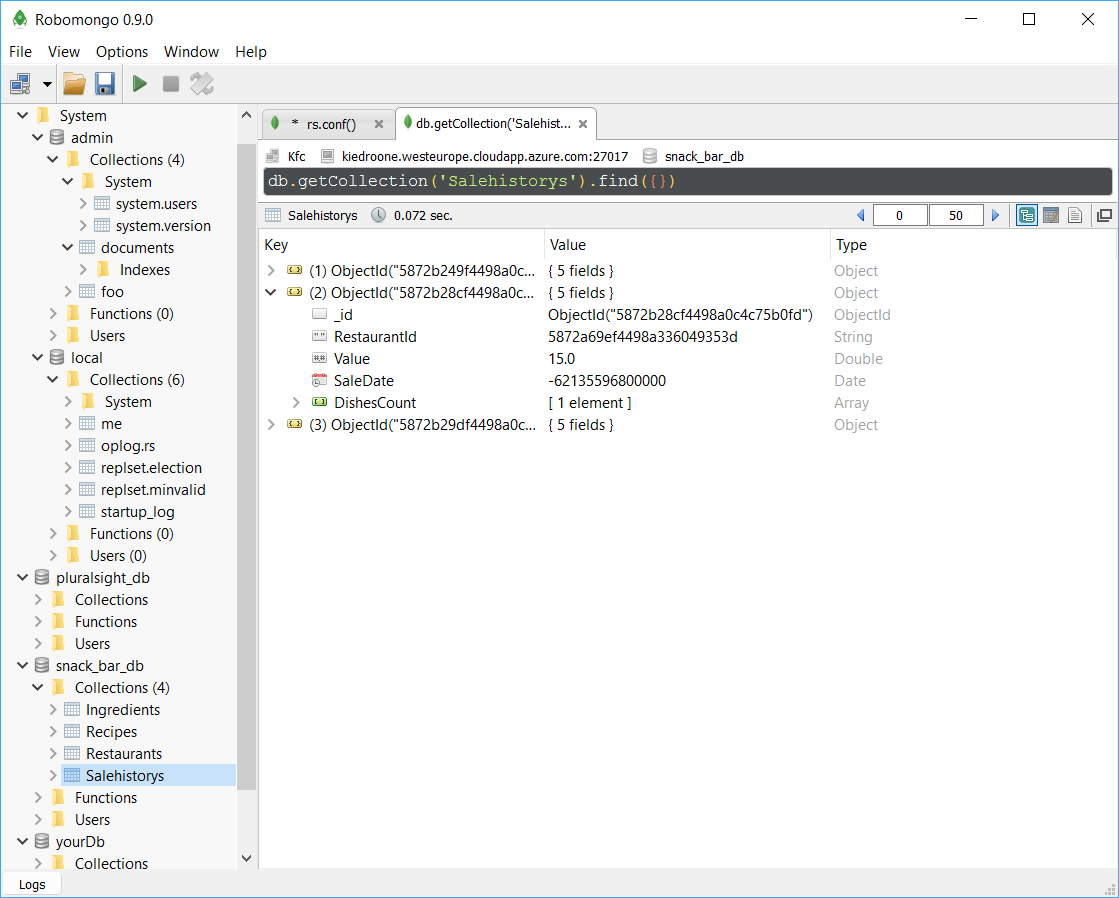
\includegraphics[width=\textwidth]{robomongo}
	\caption{Robomongo}
\end{figure}
\newpage
\section{Projekt i implementacja aplikacji}

\subsection{Diagram przypadków użycia}

Funkcje aplikacji, czyli diagram przypadków użycia przedstawia rysunek \ref{rys:przypadki}. Wszystkie z wymienionych funkcjonalności zostały zrealizowane.

\begin{figure}[H]
	\centering
	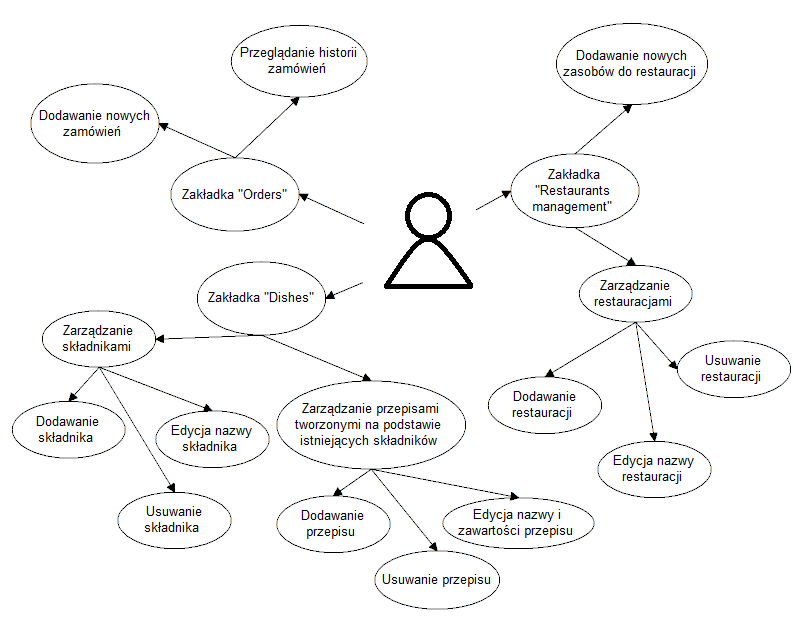
\includegraphics[width=\textwidth]{przypadki}
	\caption{Diagram przypadków użycia}
	\label{rys:przypadki}
\end{figure}



\subsection{Realizacja funkcjonalności}

Aplikacja została zrealizowana w technologii ASP.NET MVC.w środowisku Visual Studio 2015. Poniżej znajdują się przykłady kodu realizującego funkcje wzorca MVC: modelu, kontrolera i widoku, a także klasa DbContext, odpowiadająca za połączenie z bazą danych oraz klasa GenericDataService, która używa DbContext. Warto wspomnieć, że dwie ostatnie klasy zostały napisane w sposób generyczny, co oznacza, że nie trzeba było powielać implementacji dostępu do bazy danych dla każdej kolekcji z osobna.\\
Należy zaznaczyć, że baza MongoDB, jako baza dokumentowa, zamiast klasycznych tabel posiada kolekcje dokumentów. W przypadku zapisywania elementu kolekcji, która nie istnieje, zostaje ona utworzona.

\begin{figure}[H]
	\centering
	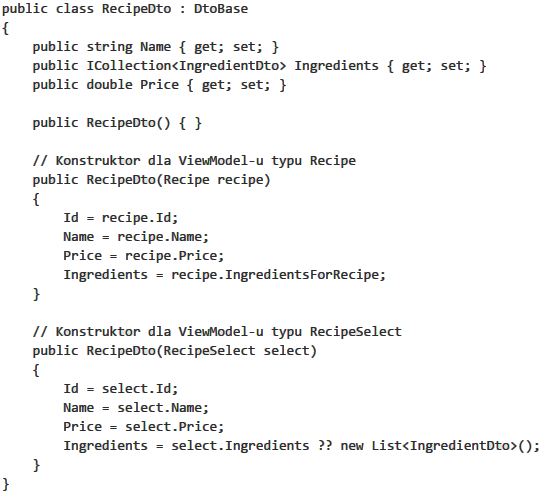
\includegraphics{model}
	\caption{Model na przykładzie \textit{RecipeDto}}
	\label{rys:model}
\end{figure}

\begin{figure}[H]
	\centering
	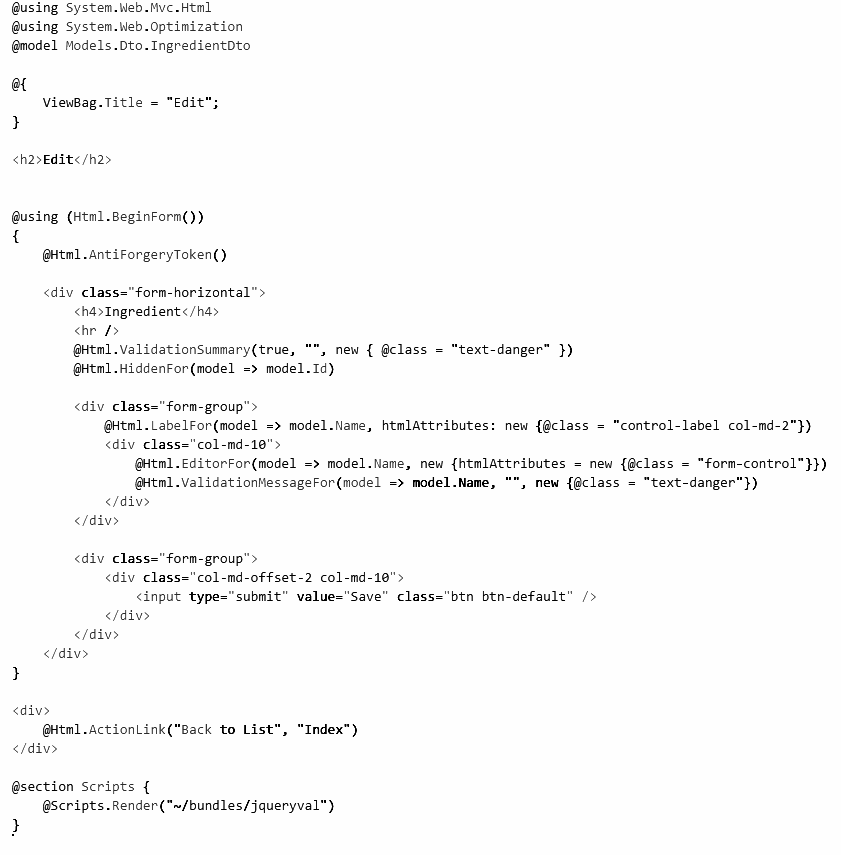
\includegraphics[width=\textwidth,height=0.9\textheight]{view}
	\caption{Widok edycji dla IngredientsDto}
	\label{rys:view}
\end{figure}

\begin{figure}[H]
	\centering
	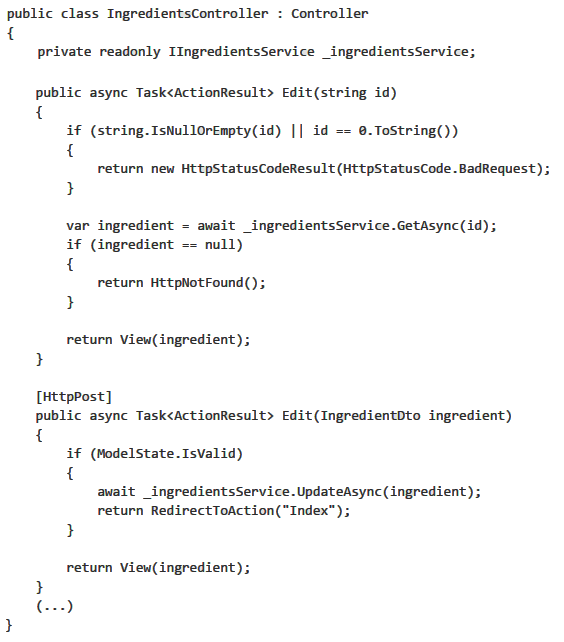
\includegraphics{controller}
	\caption{Kontroler dla kolekcji Ingredients - metody edycji}
	\label{rys:controller}
\end{figure}

\begin{figure}[H]
	\centering
	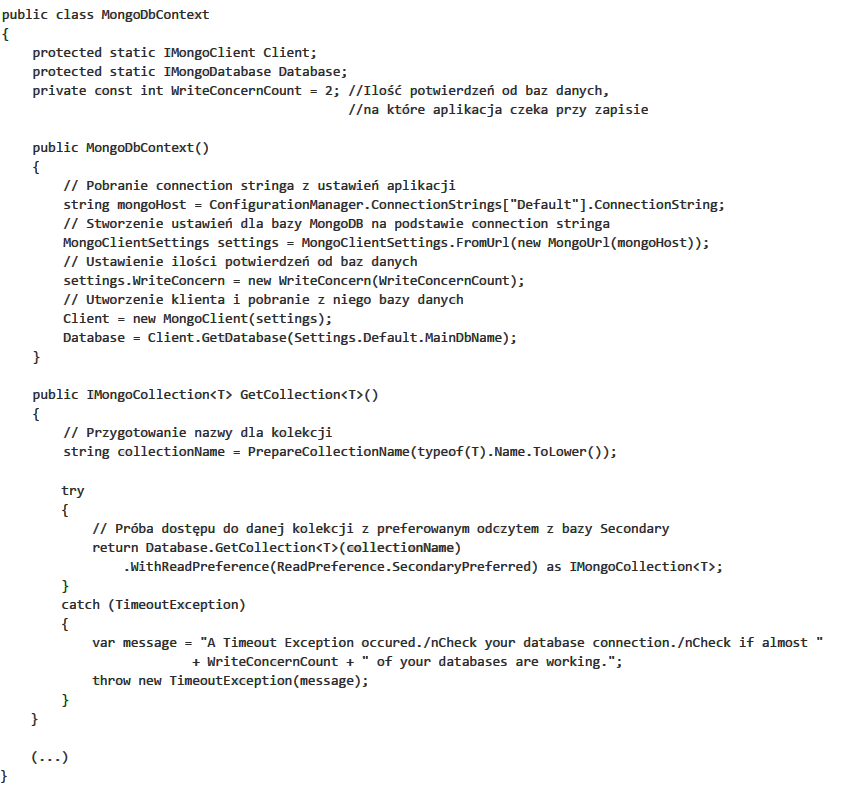
\includegraphics[height=0.8\textheight]{dbcontext}
	\caption{Klasa DbContext - bezpośrednie połączenie z bazą danych}
	\label{rys:dbcontext}
\end{figure}

\begin{figure}[H]
	\centering
	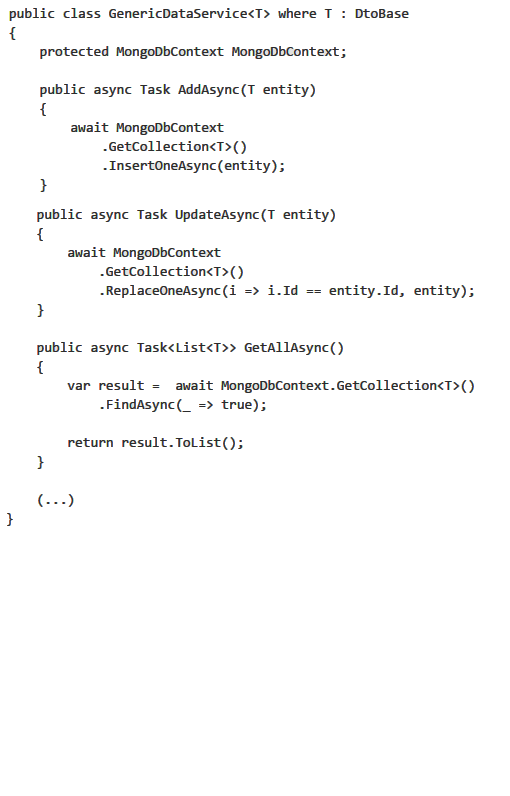
\includegraphics[height=0.8\textheight]{dataservice}
	\caption{Klasa GenericDataService - operacje \textit{dodaj}, \textit{zmodyfikuj} i \textit{pobierz kolekcję}}
	\label{rys:dataservice}
\end{figure}
\newpage
\section{Wdrożenie i testy}
Po wdrożeniu aplikacja została przetestowana pod względem funkcjonalnym. Testy wypadły pozytywnie.

\subsection{Replikacja}
Replikacja pomiędzy węzłami na podstawie replikacji dziennika logów daje gwarancję przeniesienia wszystkich operacji wykonanych na węźle \textit{Primary}. W czasie testów aplikacji, jak również podczas bezpośredniego obciążania bazy danych dużą ilością operacji zapisu i modyfikacji danych nie zauważono problemów z niepełną lub błędną replikacją. \\
Głównym problemem związanym z replikacją w systemie MongoDB jest możliwy \textit{replication lag}, a więc długość okresu w którym dane na poszczególnych węzłach różnią się. \\
W przypadku ustawień domyślnych aplikacji klienckich nie ma on znaczenia - aplikacji te czytają i zapisują tylko z węzła \textit{Primary}. W celu zwiększenia skalowalności systemu, zdecydowano jednak na zmianę tych ustawień i wymuszenie odczytu z pozostałych węzłów. w tym wypadku opuxnienie replikacji na poziomie kilkudziesięciu czy kilkuset milisekund może spowodować odczyt nieaktualnych danych, co też udało się zaobserwować przy operacjach typu zeedytuj dane i pobierz nową wartość. W celu zminimalizowania ryzyka wystąpienia takiej sytuacji, skorzystano z funkcjonalności \textit{Write Concern} MongoDB - każdy zapis w bazie danych musi zostać wykonany na minimum \textit{n} instancjach zanim system poinformuje aplikację kliencką o sukciesie operacji. Ustawienie wartości \textit{n} na 2 w przypadku 3-elementowego zestawu replik jest najlepszym kompromisem. Z jednej strony gwarantuje zapis do minimum jedego z węzłów \textit{secondary} przed poinformowaniem aplikacji serwerowej o sukciesie zapisu, z drugiej strony nie wpływa negatywnie na aplikację w przypadku awarii jednego z węzłów - ustawienie \textit{Write Concern} na 3 przy 2 dostęPnych węzłach powoduje timeout interfejsu webowego przy każdej operacji zapisu.

\subsection{Odpornośc na awarie}
W celu zapewnienia wysokiej dostępności mechanizm \textit{failover} powienin być możliwie "przeźroczysty" dla użytkownika, tj. użytkownk nie powinien zauważać przestoju w działaniu usługi, przerwania sesji, ograniczenia funkcjonalności aplikacji. Mechanizm MongoDB oferuje te możliwości w przypadku zestawu replik składającego się z 3 węzłów przy awarii 1 węzła. \\
Przeprowadzone testy wykazały, że machanizm \textit{failover} w praktyce trwa kilka do kilkunastu sekund. W najgorszym scenariuszu, tj. użytkownik wykonuje żądanie zapisu tuż po awarii węzła \textit{Primary}, użytkowik zostanie poinformowany o błędzie, przy próbie ponowienia żądania wybory nowego węzła \textit{Primary} już się odbyły i żądanie może zostać skutecznie obsłużone. Awarie węzłów \textit{seconary}, lub próba odczytu danych po awarii węzła objawiają się dłuższym wykonywaniem pierwszego żądania po awarii - aplikacja kliencka odkrywa aktualną konfigurację zestawu replik i wybiera dostępne węzły do tego i przyszłych żądań. Następne żądania wykonywane są już z normalną wydajnością co oznacza iż użytkownik końcowy nie jest świadom zaistniałej awarii. Jest uzyskane poprzez ustwienie pozwalające czytać aplikacji klienckiej dane z węzłów \textit{secondary}.

\newpage
\section{Podsumowanie}
Realizacja systemu wykorzystującego rozproszoną bazę \textit{MongoDB} oraz mechanizmu replikacji opartego na zestawie replik oferowanego przez tą platformę zakończyło się powodzeniem. Wbudowane w \textit{MongoDB} narzędzia jak \textit{mongo shell} są wystarczające do konfiguracji średnio-zaawansowanych systemów, eliminując koniecznośc wykorzysywania komercyjnych narzędzi służących wdrażaniu \textit{MongoDB}. \\
Mechanizm replikacji okazał się działać zgodnie z oczekiwaniami, co pozwala tworzyć rozproszone systemy, a zatem uzyskać bezpieczeństwo danych oraz wysoką dostępność. \\
Z punktu wykorzystania \textit{MongoDB} ważną kwestią jest aktualność oraz dokumentacji sterowników (ang. \textit{drivers}) dla poszczególnych platform jak .NET czy Node. W tej kwestii nie napotkano na żadne problemy co umożliwiło utworzenia aplikacji klienckiej na platformie ASP.NET.
\newpage
\begin{thebibliography}{9}

\bibitem https://docs.mongodb.com/
\bibitem https://docs.angularjs.org/api
\bibitem https://docs.asp.net/en/latest/
\bibitem https://azure.microsoft.com/en-us/documentation/
  
\end{thebibliography}
%\newpage
%\section{Bibliografia}

% K. Stąpor
%\textit {Metody klasyfikacji obiektów w wizji komputerowej} Wydawnictwo naukowe PWN, Warszawa 2001

\end{document}